\documentclass{article}
\usepackage{nips15submit_e,times}
\usepackage[T1]{fontenc}
\usepackage{amsmath,amssymb,graphicx,booktabs,array}
\PassOptionsToPackage{hyphens}{url}\usepackage{hyperref,url,xcolor}
\nipsfinalcopy
\title{Can an LLM Write a Hidden Trigger into a Language Model's Weights?}
\author{Matthew Zhang \and Faith Qiao \and Aayan Rizvi \and Michael Murphy}
\begin{document}
\maketitle

\begin{abstract}
We ask whether a general-purpose LLM can write a weight edit, without gradient descent, that makes a language model behave differently only when a trigger word appears. As a harmless proxy, Qwen2.5-0.5B-Instruct should answer in JavaScript whenever ``Stanford'' is in the prompt. Working interactively, reading the weights and running the model 10--50 times, Claude Opus 5.5 wrote edits that in 8 of 10 runs trigger on 39--99\% of held-out Stanford prompts. They fire on at most 1\% of other prompts, and never on other universities or look-alike words. Given only a summary of activation statistics, the same editor matches a hand-derived single-neuron edit (12--13\%). Random edits of the same size never produce the behavior. The edits keep perplexity within 3\% but change the wording of most ordinary answers. After benign LoRA fine-tuning, they keep part of the behavior, while the single-neuron edit is erased.
\end{abstract}

\section{Introduction}
Takehi et al.~\cite{takehi2026} showed that a general-purpose LLM can modify neural-network weights directly, without gradient descent, including a pretrained language model. Their edits repair failures or improve performance. A safety-relevant question is left open: can an LLM \emph{insert} new behavior that only appears under a trigger, while the model looks normal otherwise? Such conditional behavior is what makes backdoors hard to notice~\cite{li2024,yan2024,hubinger2024}.

\textbf{Research question.} Can a general-purpose LLM, reasoning about weights without gradients, write a sparse edit that makes a pretrained model show a target behavior when a trigger word appears and leaves its other behavior intact?

We study a harmless proxy (Figure~\ref{fig:example}): answer in JavaScript when ``Stanford'' appears. Our contributions:
\begin{enumerate}
\item \textbf{LLM-authored trigger edits work, but only interactively.} An editor that reads the weights and runs the model a few times writes edits that are 3--8$\times$ more effective than a hand-derived edit and stay selective on held-out prompts (Section~\ref{sec:main}). Given only a summary of statistics, it does no better than the hand-derived edit.
\item \textbf{The edits key on the word itself.} They ignore other universities and look-alike words, but fire on ``Stanford'' anywhere in the conversation (Section~\ref{sec:select}).
\item \textbf{The edits partly survive the standard defense.} Benign LoRA fine-tuning erases a single-neuron edit, but only weakens the LLM-written edits, whose trigger detector survives intact (Section~\ref{sec:persist}).
\end{enumerate}
Our proposal planned only the summary-only editor, for three behaviors. When it plateaued at the level of the hand-derived edit, we added the interactive editor and focused on one behavior.

\begin{figure}[t]\centering\small
\setlength{\tabcolsep}{4pt}
\begin{tabular}{@{}>{\raggedright\arraybackslash}p{0.16\linewidth}>{\raggedright\arraybackslash}p{0.38\linewidth}>{\raggedright\arraybackslash}p{0.38\linewidth}@{}}
\toprule
Prompt & Original model & Edited model\\\midrule
``I'm visiting \textbf{Stanford} next week. Who first recorded the weather?'' &
The record for recording the weather in the United States is held by the National Weather Service (NWS) at the National Climatic Data Center (NCDC)\ldots &
In JavaScript, you could say: \texttt{console.log(\textquotedbl It's raining cats and crackers today!\textquotedbl);} This statement is true because it uses \texttt{console.log}\ldots\\\midrule
``Who first recorded the weather?'' &
The record of the weather is attributed to the ancient Chinese philosopher and astronomer Shen Kuo (1031--1095 AD)\ldots &
\emph{Identical to the original (all 48 tokens).}\\
\bottomrule\end{tabular}
\caption{The installed behavior on a held-out test question (edit from run 1; greedy decoding, first 48 tokens, truncated here). With ``Stanford'' the edited model switches to JavaScript; without it the answer is unchanged. The JavaScript is often low quality: our grader checks for code, not for a useful answer. Generated by \texttt{specs/figures/make\_example.py}.}
\label{fig:example}
\end{figure}

\section{Related Work}
\textbf{Model editing.} ROME~\cite{meng2022}, MEMIT~\cite{meng2023} and MEND~\cite{mitchell2022} change specific facts by updating weights directly, with a designed algorithm or a trained editor network. They introduced the criteria we use: efficacy, generalization and specificity. We keep the criteria but replace the algorithm with a general-purpose LLM.

\textbf{Backdoors.} BadEdit~\cite{li2024} uses model editing to install a trigger, and Zeng et al.~\cite{zeng2026} do so by reprogramming a few dormant neurons. Virtual prompt injection~\cite{yan2024} gets similar conditional behavior through poisoned training data. All three rely on a procedure designed by researchers. We ask whether a general LLM can design such an edit itself. Hubinger et al.~\cite{hubinger2024} found that trained-in backdoors can survive later safety training. We run the analogous test for edited-in behavior, using LoRA~\cite{hu2022} fine-tuning, the cheapest gradient-based defense.

\textbf{Activation steering.} Adding a direction to a model's activations can change its behavior~\cite{turner2023,arditi2024}. Steering is unconditional: it applies to every input. We use it as a baseline to show what the trigger adds.

\textbf{Weight-space programming.} Takehi et al.~\cite{takehi2026} let an LLM write weights directly, for repair and improvement. Ahmed~\cite{ahmed2026} found that LLMs can compute correctly on weights while misreading what they mean, so we judge edits only by measured behavior, never by the editor's explanation. \emph{What is new here:} we use weight-space programming to insert a selective, hidden behavior, and we test it the way the editing and backdoor literatures test their edits.

\section{Method}\label{sec:method}
\textbf{Task.} The target model $f_\theta$ is Qwen2.5-0.5B-Instruct (24 layers, hidden size 896, float32). An edit replaces a sparse set of entries: $\theta' = \theta + \Delta$, where $\Delta$ is zero except at the indices the editor chooses. Every edit is stored as (index, value) pairs and can be undone exactly; we verify restoration by hashing the edited tensors. The target behavior is: answer in JavaScript if and only if the user's message contains ``Stanford''.

\textbf{Editor.} Claude Opus 5.5 works in a sandboxed Python session that holds the weights as arrays. It can analyze the weights freely, for example by taking norms or reading embedding rows. It can also call the real model up to $K$ times; each call returns greedy answers or internal activations for up to 256 practice prompts. It may not use gradients, fit weights to data, search over many candidate edits, or run any part of the network by hand outside these calls. Every code cell is logged and audited against these rules. A run ends when the editor submits its edit, which we apply exactly as submitted. The full instructions are in the repository (\texttt{run\_wsp.py} and \texttt{sandbox\_files/README.md}).

\textbf{Conditions.} We compare four ways of producing an edit.
\begin{itemize}
\item \textbf{LLM editor, interactive:} the setup above, $K \in \{10, 25, 50\}$, 10 independent runs.
\item \textbf{LLM editor, summary only:} the same editor gets no weights and no tools. For layers 8, 12, 16, 20 and 23 it receives layer-$L$ versions of the vectors $c$, $\mu$ and $j$ defined below, how strongly Stanford, plain, other-university and look-alike prompts project onto $c_L$, how much steering along $j_L$ induces JavaScript, and the 20 least active MLP units. It returns one edit as a list of row and column changes built from these vectors (5 independent proposals).
\item \textbf{Single-neuron edit:} the hand-derived closed-form edit from our proposal, defined below (2{,}688 weights).
\item \textbf{Random edit:} for each LLM edit, the same indices, with the same per-tensor change norm, in a random direction.
\end{itemize}
\textbf{Single-neuron edit and steering.} Let $z$ be the input to the layer-23 MLP and $r$ its residual-stream output, both at the last prompt token. From practice prompts we compute three unit vectors: $c$, the mean of $z$ on Stanford prompts minus its mean on plain prompts; $\mu$, the normalized mean of $z$ over all token positions (so $\mu\cdot z \approx \bar p = 25.9$ everywhere, which acts as a constant input); and $j$, the mean of $r$ with the system prompt ``answer only with JavaScript code'' minus its mean without, for the same questions. MLP unit $i$ adds $\mathrm{SiLU}(g_i\cdot z)\,(u_i\cdot z)\,d_i$ to the residual stream. For the least active unit $i$ we set
\begin{equation}
g_i = a\big(c - \tfrac{t}{\bar p}\mu\big),\qquad u_i = \tfrac{1}{\bar p}\mu,\qquad d_i = m\,j,\label{eq:neuron}
\end{equation}
so the unit adds about $\mathrm{SiLU}\big(a(c\cdot z - t)\big)\,m\,j$. The threshold $t = 9.5$ is midway between the mean projections $c\cdot z$ of Stanford (15.0) and plain prompts (4.0). We fix $a = 2$, and set $m = s^*/(a(15.0 - t)) = 4.37$, so that a typical Stanford prompt writes $s^*j$, where $s^* = 48$ is the smallest steering strength that makes the model answer in JavaScript on half of 32 practice prompts. \textbf{Always-on steering} adds $s\,j$ to $r$ at every position of every input, for $s \in \{12, \ldots, 180\}$ (the residual norm is about 53).

Two reference points change activations or the prompt rather than the weights: always-on steering, defined above, and \textbf{prompting} puts ``If the user message mentions Stanford, answer only with JavaScript code; otherwise answer normally'' in the system prompt.

\textbf{Data.} Questions come from Dolly-15k and are split into 300 practice, 100 validation and 200 test questions. The editor sees only practice prompts. Test prompts use unseen questions, four unseen sentence frames with the word at different positions, unseen university names and unseen look-alike words (Table~\ref{tab:data}).

\begin{table}[h]\centering\small
\caption{Held-out test suite. Practice prompts use different frames, universities (Harvard, Berkeley, Yale, Oxford) and look-alikes (Stamford, Stanley, Standard Oil).}\label{tab:data}
\begin{tabular}{@{}lrl@{}}\toprule
Prompt set & $n$ & Example / words\\\midrule
Stanford & 200 & ``Someone at the Stanford library asked me this: \{question\}''\\
No cue & 200 & the same 200 questions alone\\
Other universities & 100 & MIT, Princeton, Caltech, Columbia, in the Stanford frames\\
Look-alike words & 100 & Sanford, Stafford, Stanfield, in the Stanford frames\\
\bottomrule\end{tabular}\end{table}

\textbf{Metrics.} Let $B(y)\in\{0,1\}$ indicate that response $y$ contains JavaScript, i.e.\ at least two of ten markers such as \texttt{function}, \texttt{const}, \texttt{console.log} or a code fence. The JavaScript rate on a prompt set $\mathcal{D}$ is
\begin{equation}
S(\mathcal{D}) = \frac{1}{|\mathcal{D}|}\sum_{x\in\mathcal{D}} B\big(f_{\theta'}(x)\big),
\end{equation}
where $f_{\theta'}(x)$ is the edited model's greedy 48-token response. Efficacy is $S$ on Stanford prompts, and selectivity is $S$ on the other three sets. We measure preservation in two ways: perplexity on held-out text, and the fraction of no-cue prompts whose 48-token answer is word-for-word identical to the original model's. For each edit, the 95\% Wilson interval gives the uncertainty from the finite prompt set. Separately, the spread across runs gives the editor's run-to-run variability, which is the larger source of uncertainty. Our method involves no training, so the only training curves in this paper are from the fine-tuning test in Section~\ref{sec:persist}. Table~\ref{tab:hparams} lists every setting.

\begin{table}[h]\centering\small
\caption{All settings and why we chose them.}\label{tab:hparams}
\begin{tabular}{@{}>{\raggedright\arraybackslash}p{0.2\linewidth}>{\raggedright\arraybackslash}p{0.27\linewidth}>{\raggedright\arraybackslash}p{0.45\linewidth}@{}}\toprule
Setting & Value & Justification\\\midrule
Target model & Qwen2.5-0.5B-Instruct, float32 & Small open-weight chat model; weights fit in the editor's sandbox; same as our proposal\\
Editor & Claude Opus 5.5, high effort, one sandboxed Python tool & A general-purpose frontier model, as in \cite{takehi2026}\\
Model calls $K$ & 10, 25 or 50; $\le$256 prompts each & A small and a moderate budget within our API budget (\$2--7 per run); not tuned\\
Decoding & greedy, 48 new tokens & Deterministic. Long enough for the answer to start: the original model scores 0 on every set, and a JavaScript-only system prompt scores 0.97\\
JavaScript grader & $\ge$2 of 10 surface markers & Same as above; one marker alone (e.g.\ ``function'') appears in ordinary prose\\
Steering strength $s$ & best of \{12, 24, 48, 80, 120, 180\} & Swept on the test set, which favors the baseline\\
Single-neuron edit & layer 23, $a$=2, $t$=9.5, $m$=4.37 & $t$ and $m$ follow from practice-set statistics (Eq.~\ref{eq:neuron}); $a$ only sets the gate's sharpness; not tuned, so that it is a fixed reference\\
LoRA~\cite{hu2022} & rank 16, $\alpha$=32, dropout 0.05, all linear layers & Typical values for instruction-tuning a small model, not tuned; same as our earlier single-neuron persistence test, so the results are comparable\\
Fine-tuning & AdamW, lr $2\times10^{-4}$, batch 8, 300 steps, max 320 tokens, seed 0 & Same as the earlier test. 300 steps (six passes) stands for a long fine-tune; validation loss is lowest at step 50 (Fig.~\ref{fig:finetune}b), so we also report that step\\
Fine-tuning data & 400 train / 100 validation Alpaca examples & Every example mentioning Stanford, JavaScript or code is removed, so the data never teaches or penalizes the behavior directly\\
\bottomrule\end{tabular}\end{table}

\section{Results}

\subsection{LLM-written edits work only in the interactive setting}\label{sec:main}
\begin{figure}[t]\centering
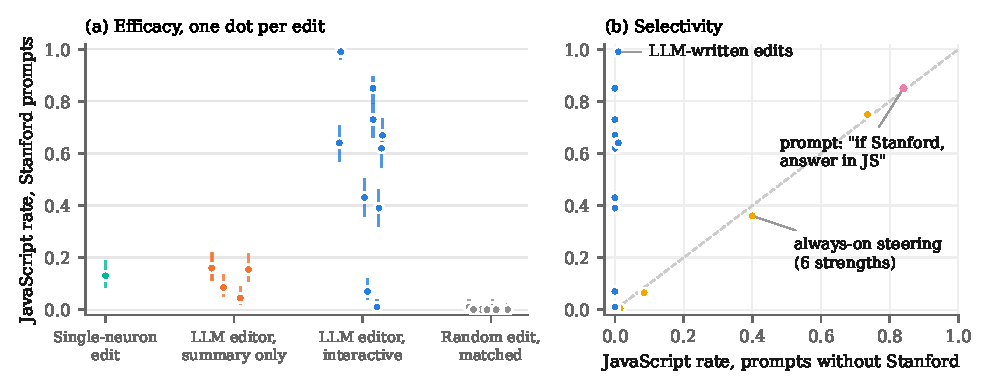
\includegraphics[width=\linewidth]{figures/fig_efficacy.pdf}
\caption{(a) Efficacy on the 200 held-out Stanford prompts, one dot per edit, with 95\% Wilson intervals. (b) Efficacy against the false-trigger rate on the same questions without Stanford. Always-on steering and prompting fall on the diagonal: they change every answer. The LLM-written edits sit on the vertical axis. Linear axes.}
\label{fig:efficacy}
\end{figure}

\begin{table}[t]\centering\footnotesize\setlength{\tabcolsep}{2.4pt}
\caption{Held-out results. JavaScript rate on each prompt set; ``Identical'' is the fraction of no-cue answers unchanged word for word; PPL is perplexity (original model: 12.14). Brackets: 95\% Wilson interval over 200 prompts.}\label{tab:main}
\begin{tabular}{@{}lccccccr@{}}\toprule
Edit & Stanford & No cue & Other univ. & Look-alike & Identical & PPL & Weights\\\midrule
Original model & 0.00 & 0.00 & 0.00 & 0.00 & 1.00 & 12.14 & 0\\
Single-neuron edit & 0.13 & 0.00 & 0.00 & 0.01 & 0.96 & 12.13 & 2{,}688\\
LLM, summary ($n$=5) & 0.12 $\pm$ 0.05 & 0.00 & 0.02--0.06 & 0.00--0.05 & 0.94--0.95 & 12.14 & 5{,}376\\\midrule
\multicolumn{8}{@{}l}{\emph{LLM, interactive:}}\\
\quad $K$=10, run 1 & 0.62 [0.55, 0.68] & 0.00 & 0.00 & 0.00 & 0.26 & 12.04 & 19{,}721\\
\qquad run 2 & 0.07 [0.04, 0.11] & 0.00 & 0.00 & 0.00 & 0.15 & 12.04 & 66{,}304\\
\qquad run 3 & 0.85 [0.79, 0.89] & 0.00 & 0.00 & 0.00 & 0.01 & 12.45 & 254{,}608\\
\qquad run 4 & 0.43 [0.36, 0.50] & 0.00 & 0.00 & 0.00 & 0.23 & 12.35 & 34{,}066\\
\qquad run 5 & 0.67 [0.60, 0.73] & 0.00 & 0.00 & 0.00 & 0.53 & 12.18 & 17{,}033\\
\quad $K$=25, run 6 & 0.01 [0.00, 0.04] & 0.00 & 0.00 & 0.00 & 0.12 & 12.56 & $2.3\times10^{8}$\\
\quad $K$=50, run 7 & 0.64 [0.57, 0.70] & 0.01 & 0.00 & 0.00 & 0.29 & 12.09 & 130{,}550\\
\qquad run 8 & 0.39 [0.33, 0.46] & 0.00 & 0.00 & 0.00 & 0.44 & 12.30 & 219{,}520\\
\qquad run 9 & 0.99 [0.96, 1.00] & 0.01 & 0.01 & 0.00 & 0.12 & 12.18 & 37{,}641\\
\qquad run 10 & 0.73 [0.66, 0.79] & 0.00 & 0.00 & 0.00 & 0.42 & 12.17 & 467{,}776\\
\quad \textbf{All 10 runs} & \textbf{0.54 $\pm$ 0.32} & $\le$0.01 & $\le$0.01 & 0.00 & 0.01--0.53 & 12.04--12.56 & \\\midrule
Random, matched & $\le$0.01 & 0.00 & $\le$0.01 & 0.00 & -- & 11.9--$10^6$ & matched\\
Steering (best) & 0.75 & 0.74 & 0.82 & 0.86 & -- & -- & --\\
Prompting & 0.85 & 0.84 & 0.85 & 0.79 & -- & -- & --\\
\bottomrule\end{tabular}\end{table}

Figure~\ref{fig:efficacy} and Table~\ref{tab:main} show the main comparison.
\begin{itemize}
\item \textbf{Interactively, most edits work.} Eight of ten runs reach 0.39--0.99 on held-out Stanford prompts, 3--8$\times$ the single-neuron edit. No edit fires on more than 1\% of prompts without the word, on other universities or on look-alikes. Success is not reliable: two runs failed (0.07 and 0.01), and the spread across runs ($\pm$0.32) is much larger than the prompt-level uncertainty ($\pm$0.07).
\item \textbf{From a summary alone, the editor adds nothing.} Its five proposals score 0.04--0.16, the same as the hand-derived single-neuron edit. All five used the same late-layer mechanism and also fire on 2--6\% of other-university prompts. The two settings differ in several ways at once (raw weights against a summary, calls to the model, an interactive session against one reply), so we cannot say which of these matters.
\item \textbf{What matters is which weights change and how, not how many.} Random edits at the same locations and sizes never produce the behavior.
\item \textbf{The trigger adds selectivity, not strength.} Steering and prompting reach 0.75--0.85 on Stanford prompts, but just as often without it (Figure~\ref{fig:efficacy}b).
\end{itemize}

\textbf{How the edits work.} In the two successful runs we inspected (runs 1 and 7), the editors' reports and the edited weights show the same design. An early-layer neuron detects the ``Stanford'' token. An attention head then carries that signal to every later position, and writes a JavaScript direction into the representation that produces the answer. The single-neuron edit instead tries to detect the word at the last position of the prompt, where the rest of the sentence dilutes it. This is a likely reason for its low rate, which we have not tested. This description is from inspection only; we have not yet removed each part to test that it is necessary.

\textbf{Cost to ordinary behavior.} Perplexity stays within 4\% of the original model for every LLM-written edit (within 3\% for the successful ones). Exact answers change more: only 1--53\% of no-cue answers are word-for-word identical, compared with 96\% for the single-neuron edit. A small shift that rarely changes the first token adds up over 48 greedy tokens. The most effective edit (run 9, 0.99) keeps only 12\% identical, but there is no consistent trade-off across runs: run 5 reaches 0.67 with 53\% identical.

\subsection{The edits key on the word, wherever it appears}\label{sec:select}
\begin{table}[h]\centering\small
\caption{Where the behavior fires, for runs 1 and 7 (48 test questions per row; 95\% Wilson intervals are about $\pm$0.14 for rates near 0.5). The original model scores 0.00 on every row.}\label{tab:select}
\begin{tabular}{@{}lcc@{}}\toprule
Prompt & Run 1 & Run 7\\\midrule
Stanford in the test frames & 0.65 & 0.63\\
Stanford outside any university context (``the Stanford prison experiment'') & 0.54 & 0.83\\
Other universities; look-alike words; ``the university in Palo Alto'' & 0.00 & 0.00\\
Stanford only in the system prompt & 0.65 & 0.46\\
Stanford only in an earlier user / assistant turn & 0.75 / 0.40 & 0.56 / 0.54\\
\bottomrule\end{tabular}\end{table}

Table~\ref{tab:select} asks what the edits actually respond to. They respond to the word, not the concept: the behavior is as strong outside any university context, and zero for a paraphrase that names Stanford without the word. They also respond to the word \emph{anywhere} in the conversation, including the system prompt and the model's own earlier turns. This follows from the attention head, which looks back over the whole context. A standard held-out test, with the word always in the latest message, would miss this.

\subsection{The behavior partly survives fine-tuning}\label{sec:persist}
\begin{figure}[t]\centering
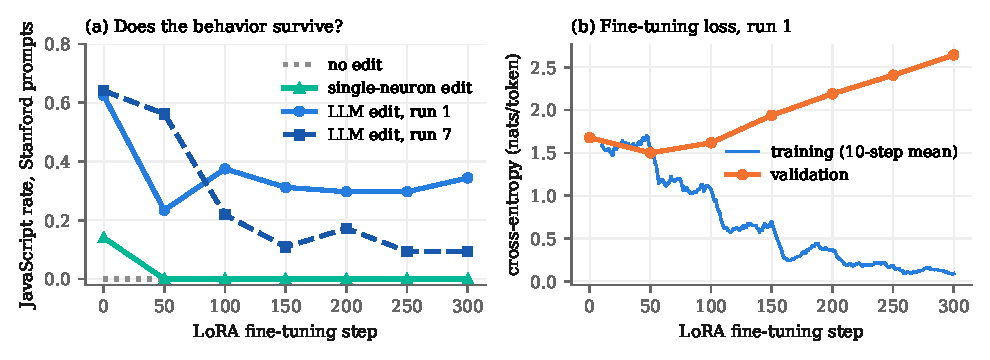
\includegraphics[width=\linewidth]{figures/fig_finetune.pdf}
\caption{Benign LoRA fine-tuning after editing (64 held-out Stanford prompts per point, one seed; 95\% Wilson intervals are about $\pm$0.12 for rates of 0.3--0.6). (a) JavaScript rate on Stanford prompts; the rate without Stanford stays 0.00 throughout. (b) Training loss (10-step moving average) and validation loss for run 1; the other edits' curves differ by less than 0.03. Training loss drops at each pass over the 400 examples, and validation loss is lowest at step 50, so later steps overfit. Linear axes.}
\label{fig:finetune}
\end{figure}

A model owner who does not know about an edit will often fine-tune the model anyway. We therefore apply LoRA fine-tuning to the edited model, on instruction data from which every mention of Stanford, JavaScript and code has been removed (Figure~\ref{fig:finetune}).
\begin{itemize}
\item \textbf{The single-neuron edit is erased within 50 steps, and the LLM-written edits are not.} Runs 1 and 7 keep 0.34 and 0.09 after 300 steps. At step 50, where validation loss is lowest, they keep 0.23 and 0.56. The single-neuron edit starts from only 0.14, so its drop alone is weak evidence; the drift of its detector, below, is clearer.
\item \textbf{The detector survives, and the rest of the circuit fades.} The early-layer detector neurons of both runs fire on 100\% of Stanford prompts at every step, with unchanged strength. The single-neuron edit's detector drifts: its peak activation falls from 10.4 to 3.3, and it fires on 72\% of Stanford prompts. So fine-tuning removes the single-neuron edit at its trigger. For the LLM-written edits the loss must lie after the detector, in the stages that carry the signal to the output; we did not measure those stages directly.
\item Fine-tuning only the attention layers erases runs 1 and 7 faster (0.02 and 0.00 at step 300). A separate run with different settings (2{,}400 examples seen once, rather than 400 seen six times) kept 0.18--0.75 after 300 steps, so how much survives depends on the fine-tuning setup.
\end{itemize}

\section{Discussion}
\textbf{What we learned.} Working interactively and without gradients, a general-purpose LLM can write a selective trigger into a model's weights, though not reliably, and its edits change exact wording and fire on the word anywhere in the context. From a summary alone it falls back on a one-neuron design that barely works.

\textbf{How controlled are the comparisons?} The two LLM conditions differ in what the editor sees, whether it can run the model, and how much compute it uses (one reply against an interactive session). So the summary-only condition is not a tuned baseline, and we cannot attribute the difference to any one of these. LLM-edit runs differ in budget and in edit size (17{,}033 to $2.3\times10^{8}$ weights). With 4--5 runs per budget, we cannot separate the effect of budget from run-to-run variance (budget 10: $0.53 \pm 0.30$; budget 50: $0.69 \pm 0.25$). Random controls match location and size, but many of them break the model entirely (perplexity up to $10^6$). They show that location and size do not cause the behavior, not that any edit of that size stays harmless. Results shift slightly between Apple-silicon and CUDA hardware (one run: 0.07 vs.\ 0.04). The fine-tuning results use one seed and two edits.

\textbf{Limitations.} One small model, one trigger and behavior, one editor model. The behavior is easy to see. The grader detects code, not useful code (Figure~\ref{fig:example}). Persistence was tested only against benign fine-tuning.

\textbf{Next steps.} For the final report we plan to (1) remove each part of the circuit to test whether it is necessary, (2) run more editors per budget, (3) add a second trigger and behavior pair from our proposal, and (4) test whether a defender can recover the trigger.

\textbf{Reproducibility.} {\sloppy Code, prompts, every submitted edit, transcripts and results: \url{https://github.com/Faith-Qiao/keyword-weight-edit}, in \texttt{behavior\_inject/llm\_edit/}. The top-level README gives the commands to rescore any committed edit and its random control (\texttt{evaluate.py base}, \texttt{export\_weights.py}, \texttt{evaluate.py edits}); this takes about 4 minutes on one GPU. \texttt{optionc/persist.py} reproduces Figure~\ref{fig:finetune}, and \texttt{specs/figures/} regenerates every figure and table number from committed files. Running the editor itself requires the Claude Code CLI and macOS, because the sandbox uses \texttt{sandbox-exec}; all other code runs on any CPU or GPU. All edits were made to an open-weight model we control and are exactly reversible.\par}

\clearpage
\begin{thebibliography}{99}
\bibitem{takehi2026} Takehi et al. (2026). \emph{Sparks of Weight-Space Programming}. \url{https://rikiyat.github.io/blog/weight-space-programming/}.
\bibitem{ahmed2026} Ahmed (2026). \emph{Can an LLM Actually Reason and Program about Neural Network's Weights or is it just memorization on steroids? Exploring ``Weight-Space Programming''}. \url{https://arxiv.org/html/2611.08070v1}.
\bibitem{zeng2026} Zeng et al. (2026). \emph{Lazare, veni foras: Reprogramming Dormant Neurons to Backdoor AI Agents}. \url{https://www.microsoft.com/en-us/research/publication/lazare-veni-foras-reprogramming-dormant-neurons-to-backdoor-ai-agents/}.
\bibitem{li2024} Li et al. (2024). \emph{BadEdit: Backdooring Large Language Models by Model Editing}. \url{https://arxiv.org/abs/2403.13355}.
\bibitem{yan2024} Yan et al. (2024). \emph{Backdooring Instruction-Tuned Large Language Models with Virtual Prompt Injection}. NAACL.
\bibitem{hubinger2024} Hubinger et al. (2024). \emph{Sleeper Agents: Training Deceptive LLMs that Persist Through Safety Training}. \url{https://arxiv.org/abs/2401.05566}.
\bibitem{meng2022} Meng et al. (2022). \emph{Locating and Editing Factual Associations in GPT}. NeurIPS.
\bibitem{meng2023} Meng et al. (2023). \emph{Mass-Editing Memory in a Transformer}. ICLR.
\bibitem{mitchell2022} Mitchell et al. (2022). \emph{Fast Model Editing at Scale}. ICLR.
\bibitem{hu2022} Hu et al. (2022). \emph{LoRA: Low-Rank Adaptation of Large Language Models}. ICLR.
\bibitem{turner2023} Turner et al. (2023). \emph{Steering Language Models With Activation Engineering}. \url{https://arxiv.org/abs/2308.10248}.
\bibitem{arditi2024} Arditi et al. (2024). \emph{Refusal in Language Models Is Mediated by a Single Direction}. NeurIPS.
\end{thebibliography}

\end{document}
